\chapter{Implementacija i korisničko sučelje}
		
		
		\section{Korištene tehnologije i alati}
		
			
			 {Komunikacija u timu se obavljala pomoću aplikacija \underbar{WhatsApp}\footnote{Aplikacija za besplatnu razmjenu poruka, fotografija, videozapisa i drugih datoteka, te uspostavljanje glasovnih i videopoziva putem mobilnog interneta pametnim telefonima:\newline\url{https://www.whatsapp.com/}} i \underbar{Discord}\footnote{Besplatna aplikacija za komunikaciju putem tekstualnih poruka i glasovnih i video poziva:\newline\url{https://discord.com/}}.
			 	\newline Dokumentacija je bila pisana pomoću alata TeXstudio i TexLive. Za izradu UML dijagrama korišten je alat \underbar{Astah Professional}\footnote{https://astah.net/products/astah-professional/}.Kao razvojno okruženje korišten je \underbar{IntelliJ IDEA Ultimate}\footnote{https://www.jetbrains.com/lp/intellij-frameworks/}. IntelliJ IDEA je integrirano razvojno okruženje napisano u Javi za razvoj računalnog softvera napisanog u Javi, Kotlinu, Groovyju i drugim jezicima koji se temelje na JVM-u. Razvio ga je JetBrains i dostupan je u dva izdanja, Ultimate i Community. Aplikacija je napisana koristeći radni okvir \underbar{Spring Boot}\footnote{\url{https://spring.io/projects/spring-boot}} i jezik \underbar{Java}\footnote{\url{https://www.java.com/en/}} za izradu backenda. Za izradu frontenda je koristen \underbar{React}\footnote{Besplatna JavaScript biblioteka otvorenog tipa za izgradnju korisničkih sučelja:\newline\url{https://reactjs.org/}}. Za izradu naše baze podataka koristili smo \underbar{PostgreSQL}\footnote{https://www.postgresql.org/}.}
			
			
			\eject 
		
	
		\section{Ispitivanje programskog rješenja}
			
			
			TESTIRANJE SUSTAVA
			\newline \newline
			Testiranje sustava se provodi sa "Chrome-om" proširenjem „Selenium IDE“. „Selenium IDE“ je aplikacija koja nam omogućava snimanje akcija korisnika u raznim slučajevima. U nastavku su prikazani rezultati testova odabranih slučajeva koji dovode funkcionalnost našeg sustava u pitanje. 
			\newline \newline
			Testirati ćemo sustav na sljedećim testovima:
			\begin{packed_item}
				\item \textit{Logiranje u aplikaciju u slučaju da je sve ispravno napravljeno}
				\item \textit{Logiranje u aplikaciju u slučaju da je email adresa kriva}
				\item \textit{Logiranje u aplikaciju u slučaju da je lozinka kriva}
				\item \textit{Logiranje u aplikaciju u slučaju da su email i lozinka krivi}
				\item \textit{Registracija korisnika u slučaju da je sve ispravno napravljeno}
				\item \textit{Registracija već registriranog korisnika}
				\item \textit{Registracija korisnika u slučaju da je email zadan u krivom formatu}
			\end{packed_item}
			
			
			\begin{figure}[H]
				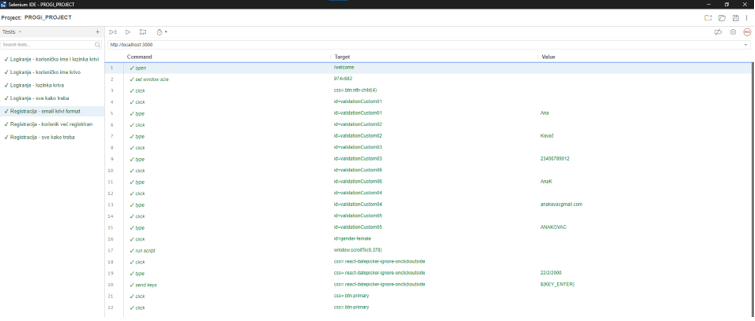
\includegraphics[scale=1]{slike/Ispit1.PNG} %veličina slike u odnosu na originalnu datoteku i pozicija slike
				\centering
				\caption{Registracija korisnika u slučaju da je email zadan u krivom formatu}
				\label{fig:promjene}
			\end{figure}
			
			
			Tijek testa: Ušli smo na pravu web adresu i kliknuli na tipku „Registracija“ nakon čega nam se otvorio novi prozor za registraciju. Upisali smo email adresu bez simbola „@“ što taj email čini nevažećim tj. krivoga formata. Sve ostale informacije su bile tehnički korektne. Rezultat jest nemogućnost registriranja zbog krivog formata email adrese.
			
			\begin{figure}[H]
				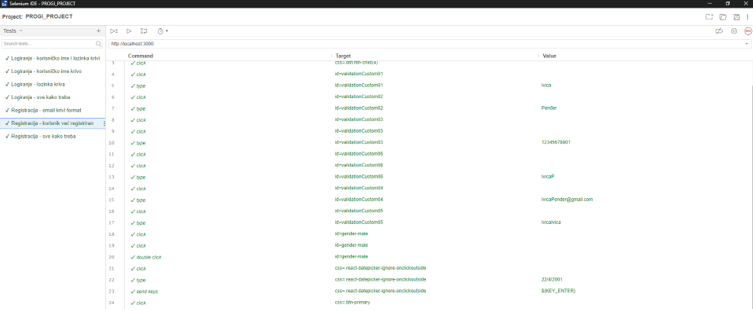
\includegraphics[scale=1]{slike/Ispit2.PNG} %veličina slike u odnosu na originalnu datoteku i pozicija slike
				\centering
				\caption{Registracija već registriranog korisnika}
				\label{fig:promjene}
			\end{figure}
			
			Tijek testa: Ušli smo na pravu web adresu i kliknuli na tipku „Registracija“ nakon čega nam se otvorio novi prozor za registraciju. Upisali smo valjane podatke „stvarne osobe“ koja je već registrirana u našoj bazi podataka. Rezultat je nemogućnost ponovnog registriranja.
			
			\begin{figure}[H]
				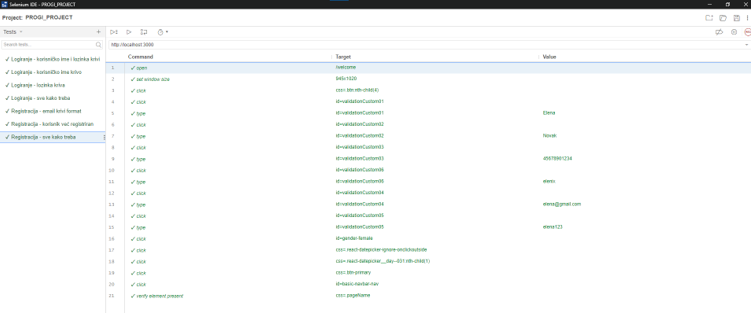
\includegraphics[scale=1]{slike/Ispit3.PNG} %veličina slike u odnosu na originalnu datoteku i pozicija slike
				\centering
				\caption{Registracija korisnika u slučaju da je sve ispravno napravljeno}
				\label{fig:promjene}
			\end{figure}
			
			Tijek testa: Ušli smo na pravu web adresu i kliknuli na tipku „Registracija“ nakon čega nam se otvorio novi prozor za registraciju. Upisali smo željene podatke „stvarne osobe“ koja još nije registrirana u našoj bazi podataka te smo se uspješno registrirali u sustav te dobili pristup stranici „Prijava“.
			
			\begin{figure}[H]
				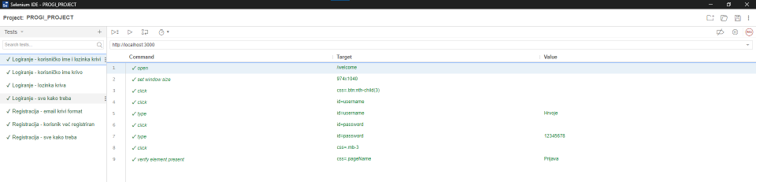
\includegraphics[scale=1]{slike/Ispit4.PNG} %veličina slike u odnosu na originalnu datoteku i pozicija slike
				\centering
				\caption{Logiranje u aplikaciju u slučaju da su korisničko ime i lozinka krivi}
				\label{fig:promjene}
			\end{figure}
			
			Tijek testa: Ušli smo na pravu web adresu i kliknuli na tipku „Prijava“ nakon čega nam se otvorio novi prozor za prijavu u sustav. Upisali smo podatke izmišljenog računa – korisničko ime i lozinku koji ne postoje. Rezultat je nemogućnost prijave u sustav. 
			\begin{figure}[H]
				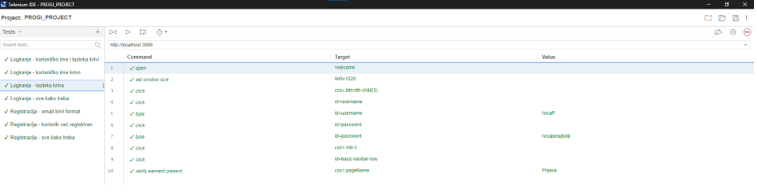
\includegraphics[scale=1]{slike/Ispit5.PNG} %veličina slike u odnosu na originalnu datoteku i pozicija slike
				\centering
				\caption{Logiranje u aplikaciju u slučaju da je lozinka kriva}
				\label{fig:promjene}
			\end{figure}
			
			Tijek testa: Ušli smo na pravu web adresu i kliknuli na tipku „Prijava“ nakon čega nam se otvorio novi prozor za prijavu u sustav. Upisali smo postojeće korisničko ime ali krivu lozinku koja nije povezana s tim korisničkim imenom. Rezultat je nemogućnost prijave u sustav. 
 
				\begin{figure}[H]
				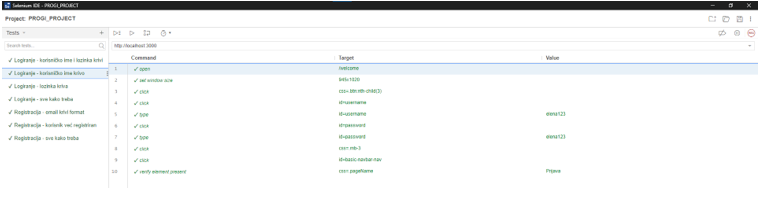
\includegraphics[scale=1]{slike/Ispit6.PNG} %veličina slike u odnosu na originalnu datoteku i pozicija slike
				\centering
				\caption{Logiranje u aplikaciju u slučaju da je korisničko ime krivo}
				\label{fig:promjene}
			\end{figure}
			
			Tijek testa: Ušli smo na pravu web adresu i kliknuli na tipku „Prijava“ nakon čega nam se otvorio novi prozor za prijavu u sustav. Upisali smo lozinku koja se nalazi u sustavu ali korisničko ime se ne podudara onim povezanim sa lozinkom. Rezultat je nemogućnost prijave u sustav. 
			
			\begin{figure}[H]
				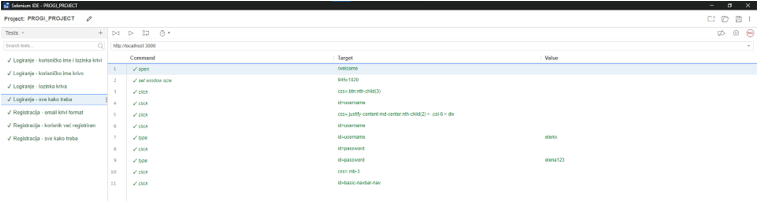
\includegraphics[scale=1]{slike/Ispit7.PNG} %veličina slike u odnosu na originalnu datoteku i pozicija slike
				\centering
				\caption{Logiranje u aplikaciju u slučaju da je sve ispravno napravljeno}
				\label{fig:promjene}
			\end{figure}
			
			Tijek testa: Ušli smo na pravu web adresu i kliknuli na tipku „Prijava“ nakon čega nam se otvorio novi prozor za prijavu u sustav. Upisali smo potrebne podatke – postojeće korisničko ime i pripadnu lozinku. Rezultat je uspješna prijava u sustav i preusmjeravanje na novu stranicu „Pacijent“ (uloga ovog korisnika je „Pacijent“, da se prijavio korisnik sa ulogom „Admin“ bio bi preusmjeren na novu stranicu „Admin“).
				\eject
		
		
		\section{Dijagram razmještaja}
			
		U ovom dijagramu razmještaja opisana je programska potpora i topologija sklopov-
		lja korištena u radnom okruženju sustava. Sustav je izveden u arhitekturi ”klijent-
		poslužitelj” i podijeljen je na dva dijela, na poslužiteljsko i korisničko računalo.
		Baza podataka i web poslužitelj nalaze se na poslužiteljskom računalu, klijent se
		koristi web preglednikom kako bi pristupio web aplikaciji, a sva komunikacija
		izmedu klijenta i poslužitelja odvija se HTTPS vezom.
		
		\begin{figure}[H]
			\includegraphics[scale=0.8]{slike/Dijagram razmještaja.PNG} %veličina slike u odnosu na originalnu datoteku i pozicija slike
			\centering
			\caption{Specifikacijski dijagram razmještaja}
			\label{fig:promjene}
		\end{figure}
			
			\eject 
		
		\section{Upute za puštanje u pogon}
		
			Mi smo se odlučili dovršenu aplikaciju pokrenuti na Amazon AWS-u.
			\newline
			
	\textbf{Amazon RDS  (Relational Database Service) }
	\newline
	
	       Amazon RDS (Relational Database Service) je usluga upravljanja relacijskim bazama podataka koju pruža Amazon Web Services (AWS). Ova usluga omogućuje korisnicima lako postavljanje, upravljanje i skaliranje relacijskih baza podataka u oblaku bez potrebe za kompleksnim administrativnim zadacima.
	       
	       Nakon upisivanja potrebnih podataka (instance identifier, master username, password, port, initial database name) napravit će se naša baza podataka koja će se vrtit na javnom poslužitelju. Zatim treba SpringBoot aplikaciju povezati s tom bazom podataka.
			
			\begin{figure}[H]
				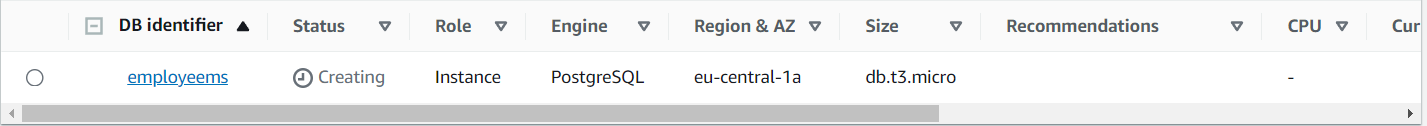
\includegraphics[scale=0.5]{slike/Deploy1.PNG} %veličina slike u odnosu na originalnu datoteku i pozicija slike
				\centering
				\caption{Stvorena instanca baze podataka}
				\label{fig:promjene}
			\end{figure}
			
				\begin{figure}[H]
				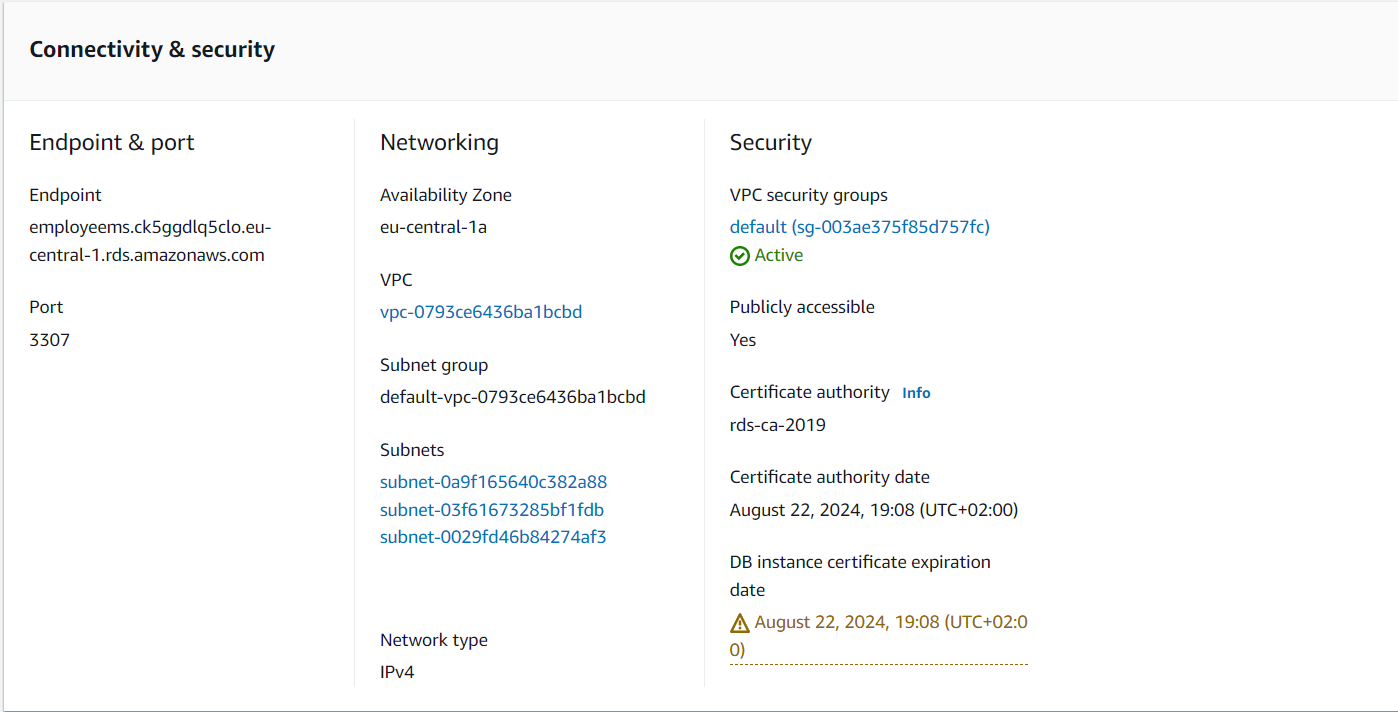
\includegraphics[scale=0.5]{slike/Deploy2.PNG} %veličina slike u odnosu na originalnu datoteku i pozicija slike
				\centering
				\caption{Podatci naše nove baze podataka}
				\label{fig:promjene}
			\end{figure}
			
			\begin{figure}[H]
				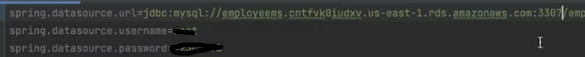
\includegraphics[scale=1]{slike/Deploy3.PNG} %veličina slike u odnosu na originalnu datoteku i pozicija slike
				\centering
				\caption{Spajanje baze podataka za backend-om}
				\label{fig:promjene}
			\end{figure}
			
				\textbf{Amazon EC2  (Elastic Compute Cloud) }
			\newline
			
			EC2 je servis u okviru AWS-a koji pruža skalabilne virtualne servere u oblaku. EC2 instance omogućavaju korisnicima da pokreću virtualne servere sa različitim konfiguracijama resursa, kao što su CPU, memorija, skladište itd.
			
			
			
			\eject 